\subsection{Hysteresekurve}
In dieser Versuchsreihe wird die Hysteresekurve mitsamt der Neukurve eines Eisenkerns in einer Toroidspule 
in Abhängigkeit der Stromstärke $I$ ermittelt.
Anhand der gemessenen Daten sollen Sättigungsmagnetisierung, Remanenz und Koerzitivkraft der Hysteresekurve bestimmt werden.
Außerdem sind differentielle Permeabilität für $H = 0$ und Sättigungswert der Neukruve zu ermitteln.

\noindent
Die Ringspule hat einen Luftspalt, damit an dieser Stelle eine transversale Hall-Sonde das Magnetfeld messen kann.
Der Anleitung wird eine Windungszahl von $n = 595$ und eine Breite des Luftspaltes von \qty[]{3}{\mm} entnommen.
Der Aufbau der Toroidspule ist weitestgehend vorbereitet, es muss nur das Spannungsgerät mit 2 Kabeln angeschlossen und die Hall-Sonde orientiert werden.
Da der Eisenkern noch eine gewisse Restmagnetisierung von vorherigen Versuchen haben kann,
wird zunächst eine Wechselspannungsquelle angeschlossen und ein starkes Wechselfeld eingestellt, um das Material zu entmagnetisieren.

\noindent
Im nächsten Schritt wird die eigentliche Spannungsquelle an die Spule angeschlossen.
Für eine Spannung $U = \qty[]{0}{\volt}$ und eine Stromstärke $I = \qty[]{0}{\ampere}$ wird der Wert der magnetischen Flussdichte abgelesen, 
die auch nach der Entmagnetisierung noch vorhanden ist.
Daraufhin wird die Stromstärke $I$ schrittweise um \qty[]{0.5}{\ampere} erhöht bis bei einem Wert von \qty[]{10}{\ampere} die Sättigung erreicht wird.
Dabei ist darauf zu achten, dass die Stromstärke nur in eine Richtung erhöht wird, um die Ergebnisse nicht zu verfälschen.
Falls also beim Erhöhen der Werte $I$ etwas zu groß eingestellt wird, darf es nicht niedriger geregelt werden.
Für jede eingestellte Stromstärke $I$ wird die magnetische Flussdichte $B$ in Abhängigkeit von $I$ notiert.
Mit Hilfe der hier gemessenen Daten können Neukurve sowie alle geforderten zugehörigen Größen ermittelt werden.

\noindent
Um die Kenngrößen der Hysteresekurve zu bestimmen, wird mit der gleichen Schrittweite $I$ stückweise bis zu \qty[]{0}{\ampere} gesenkt.
Anschließend wird umgepolt, wobei vor und nach dem Umpolen die magnetische Flussdichte für \qty[]{0}{\ampere} notiert wird.
Nach dem Umpolen wird erneut die Stromstärke bis \qty[]{10}{\ampere} erhöht und die eingestellten Werte von $I$ werden beim Notieren
mit einem negativen Vorzeichen versehen.
Anhand dieser Daten kann der obere Teil der Hysteresekurve bestimmt werden.
Der Vorgang wird wiederholt, damit auch der untere Teil der Kurve ermittelt werden kann.
Ein Foto des Versuchsaufbaus ist in Abbildung \ref{fig:hysterese_aufbau} zu sehen.


\begin{figure}[H]
    \centering
    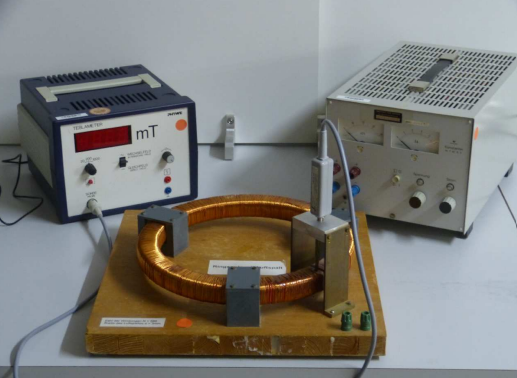
\includegraphics[]{abbildungen/toroidspule mit kern.png}
    \caption{Versuchsaufbau zur Bestimmung der Hysteresekurve \cite[]{man:v308}.}
    \label{fig:hysterese_aufbau}
\end{figure}

%Um die magnetische Flußdichte eines Toroides mit Eisenkern zu messen, muß ein Luftspalt eingefugt werden.
